\documentclass[12pt]{article}
\usepackage{verbatim}
\usepackage[dvips]{epsfig}
\usepackage{color}
\usepackage{url}
\usepackage[colorlinks=true]{hyperref}

\begin{document}

\section*{GENESIS: Documentation}

{\bf Related Documentation:}
% start: userdocs-tag-replace-items related-do-nothing
% end: userdocs-tag-replace-items related-do-nothing

\section*{De Schutter: Purkinje Cell Model}

\subsection*{Source}

De Schutter E \& Bower JM (1994) An active membrane model of the cerebellar Purkinje cell I. Simulation of current clamp in slice. {\it Journal of Nerurophysiology}. {\bf 71}: 375--400. \\

\subsection*{High-threshold Ca$^{2+}$-activated K$^+$ (KC) Current}

\begin{figure}[h]
\centering
   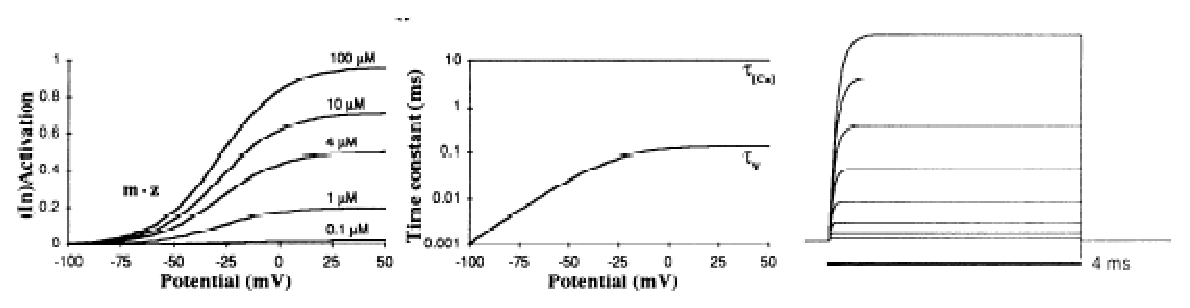
\includegraphics[scale=0.75]{figures/DS1.2G.eps}
   \caption{Activation and inactivation properties of the high-threshold Ca$^{2+}$-activated K$^+$ current (KC, ---) ionic conductances in the model. Seady-state activation and inactivation vs. voltage are plotted at the {\em left}, the time constants of activation ($\tau_m$) and inactivation ($\tau_h$) vs. voltage in the {\em middle} (Note: Semilogarithmic scale), and a simulation of representative voltage-clamp currents at the {\em right}. Note: Activation is controlled by the product of a voltage and a [Ca${2+}$]-dependent factor, each with their own time constants ($\tau_v$ and $\tau_{[Ca]}$). The voltage clamps simulate steps from a holding potential of -110 to -70\,mV up to 0\,mV in 10\,mV increments. The voltage-clamp current amplitude has been scaled arbitrarily because we mainly wanted to demonstrate the current kinetics.}
   \label{fig:DS1.2G}
\end{figure}

Ca$^{2+}$-activated K$^+$ channels are assumed to be responsible for the repolarization of dendritic Ca$^{2+}$ spikes\,\cite{R:1980pi}. Several Ca$^{2+}$-activated K$^+$ channels have been identified in single channel studies of Purkinje cells\,\cite{Gahwiler:1989fk, Gruol:1989oq, Gruol:1991dz} among them a large conductance channel corresponding to the BK or maxi-K channel\,\cite{Latorre:1989fu}. The macroscopic current carried by this channel is called the C current (KC) and is characterized by a voltage dependence and tetraethylammonium (TEA) sensitivity\,\cite{} (Adams et al. 1982). This channel is widely distributed in different tissues in both vertebrate and invertebrate preparations, with apparently similar voltage dependence but a variable Ca$^{2+}$ dependence in all the cells studied\,\cite{Latorre:1989fu}.

No experimental studies on the kinetics of KC in Purkinje cells were available. Technically it is difficult to characterize the kinetics of KC because the Ca$^{2+}$ activation cannot be controlled by a ``Ca$^{2+}$ clamp'' comparable to voltage clamps. So most experimental investigations have sacrificed temporal resolution by investigating channel activation at steady, well-controlled Ca$^{2+}$ concentrations\,\cite{McManus:1898kl, Moczydlowski:1983qa, Smart:1987mi}. Several groups that have tried to study the temporal dynamics of Ca$^{2+}$ activation, i.e., how fast the channel reacts to a sudden jump in Ca$^{2+}$ concentration, have concluded that there was a significant lag in response\,\cite{Gola:1990pi, Hudspeth:1988ff, Ikemoto:1989lh, L:1989ff}. Most reports agree that a minimal model of the BK channel requires at least three closed states and one open state, that the open-closed transitions include at least two Ca$^{2+}$ binding steps and a voltage-independent step, and that the channel does not inactivate\,\cite{Gola:1990pi, Moczydlowski:1983qa, Smart:1987mi}. However, there is no agreement on the details of these models because, for example, reported Hill coefficients for Ca$^{2+}$-dependent opening vary between 1--2\,\cite{Franciolini:1988fu, Moczydlowski:1983qa}, exactly 2\,\cite{Hudspeth:1988ff, Reinhart1989:xe} and 3\,\cite{Ikemoto:1989lh} and some authors assume more than one open state\,\cite{McManus:1898kl, Smart:1987mi}. Most BK channels studied in adult neurons require concentrations of internal Ca$^{2+}$ in the micromolar range to fully activate\,\cite{Franciolini:1988fu, Lancaster:1991ye, Reinhart1989:xe, Smart:1987mi} and the dependence on Ca$^{2+}$ concentration seems to be nonlinear\,\cite{Franciolini:1988fu, Moczydlowski:1983qa} (also see however\,\cite{L:1989ff}).

The conflicting experimental data on the BK channel are reflected by the multiple approaches used by different modelers to describe this channel. Most models lump all the open-closed transitions together into one differential equation\,\cite{hines84:_effic, Moczydlowski:1983qa, D:1982lh, Yamada-W:1989bs}. Following the example of\,\cite{Traub-R-D:1991mi} we have described this channel with two independent state variables ($m$ and $z$ in \href{pub-purkinje-deschutter-equations/pub-purkinje-deschutter-equations.tex}{\bf Eq. 1}), but we have used a different model for the Ca$^{2+}$-dependent step. The Ca$^{2+}$-independent gate was modeled along data from\,\cite{Gola:1990pi} with a voltage-independent activation ($\alpha_m$) and a voltage-dependent inactivation ($\beta_m$), with a typical 15\,mV per e-fold change in conductance\,\cite{Franciolini:1988fu, Latorre:1989fu}. We shifted the deactivation to more positive potentials to fit the strong depolarizations ($>$50 mV) required to activate KC in Purkinje cells, as reported by\,\cite{Gruol:1991dz}. The Ca$^{2+}$-binding step was modeled along\,\cite{Franciolini:1988fu} as an adsorption isotherm distribution with a half-activation at 4\,$\mu$M and a Hill coefficient of 2 (..\href{pub-purkinje-deschutter-equations/pub-purkinje-deschutter-equations.tex}{\bf Eq. 5}). The delay in activation was modeled explicitly by a time constant of activation of 10\,ms\,\cite{Gola:1990pi, Ikemoto:1989lh, L:1989ff}.

\bibliographystyle{plain}
\bibliography{../tex/bib/g3-refs}

\end{document}
